% !TEX TS-program = pdflatex
% !TEX encoding = UTF-8 Unicode



\documentclass[11pt,a4paper]{article}

%\usepackage[francais]{babel} % bug à la compilation chez moi
\usepackage[T1]{fontenc}
\usepackage[utf8]{inputenc}

\usepackage{amsmath,amsfonts,amssymb}

\usepackage{geometry}
\geometry{margin=75pt}

\usepackage[upright]{fourier}
\usepackage{subfig}

\usepackage{shadethm}

\usepackage{color}
\definecolor{gris_clair}{gray}{.9}
\definecolor{gris}{gray}{.35}
\definecolor{vert}{rgb}{0,0.5,0}
\definecolor{rouge}{rgb}{0.5,0,0}
\definecolor{turquoise}{rgb}{0,0.5,0.5}

\usepackage{listings}
\usepackage{paralist}
%\usepackage{stmaryrd} % bug à la compilation chez moi
\usepackage{tikz}
\usetikzlibrary{shapes.multipart}

\lstset{
language=Python,
backgroundcolor=\color{gris_clair},
frame=single,
basicstyle=\footnotesize\ttfamily\color{gris},
identifierstyle=\color{black},
keywordstyle=\color{vert},
stringstyle=\color{rouge}, showstringspaces=false,
commentstyle=\itshape\color{turquoise},
%numbers=left, numbersep=5pt, numberstyle=\color{gris}\tiny,stepnumber=5,
breaklines=true,
literate=
  {é}{{\'e}}1 {É}{{\'E}}1 {à}{{\`a}}1 {è}{{\`e}}1% 
  {À}{{\`A}}1 {È}{{\'E}}1 {ë}{{\"e}}1 {ï}{{\"i}}1%
  {â}{{\^a}}1 {ê}{{\^e}}1 {î}{{\^i}}1 {ô}{{\^o}}1% 
  {û}{{\^u}}1 {Â}{{\^A}}1 {Ê}{{\^E}}1 {Î}{{\^I}}1%
  {Ô}{{\^O}}1 {œ}{{\oe}}1 {Œ}{{\OE}}1 {æ}{{\ae}}1%
  {Æ}{{\AE}}1 {ç}{{\c c}}1 {Ç}{{\c C}}1 {€}{{\EUR}}1 ,
morekeywords={len,input,range}}         


\title{Correction des exercices sur le labyrinthe}
\date{}
\author{Antonin Dudermel \and Ambroise Poulet \and Matthias Goffette}

\begin{document}

\newshadetheorem{defin}{Définition}
\newshadetheorem{theo}{Théorème}

\maketitle

\begin{it}
Nous avons ici un algorithme créant un labyrinthe parfait de dimension $n$. Nous voulons le modifier, d'abord pour enegistrer le labyrinthe en une image, puis pour construire le chemin entre les cases $(0,0)$ et $(n-1,n-1)$.
\end{it}
\par
Les fonctions originales sont les suivantes :

\begin{lstlisting}
def visiter(c):
    (x,y) = c
    if x < 0 or x>= n or y<0 or y>=n:
        return
    atteinte[x][y] = True

def est_atteinte(c):
    (x,y) = c
    if x < 0 or x>= n or y<0 or y>=n:
        return True
    return atteinte[x][y]

def choix(c):
    (x,y) = c
    r = []
    def ajouter(p):
        if not est_atteinte(p):
            r.append(p)
    ajouter((x-1,y))
    ajouter((x+1,y))
    ajouter((x,y-1))
    ajouter((x,y+1))
    return r

def tirage(L):
    m = len(L)
    assert m > 0
    return L[random.randint(0, m-1)]

def labyrinthe():
    pile = creer_pile(n*n)
    empiler(pile, (0,0))
    visiter((0,0))
    while not est_vide(pile):
        cellule = depiler(pile)
        print(cellule)
        c = choix(cellule)
        if len(c) > 0:
            suivante = tirage(c)
            # c'est ici qu'on relie les cases cellule et suivante
            visiter(suivante)
            empiler(pile, cellule)
            empiler(pile, suivante)
            
atteinte = [[False] * n for i in range(n)]
\end{lstlisting}
\par
Tout d'abord, nous allons réaliser l'enregistrement du labyrinthe au format PGM. Ce format permet d'enegistrer facilement des images en nivau de gris. Pour ce faire, nous avons besoin de plusieurs modifications :
\begin{itemize}
	\item En premier lieu, il faut compléter la fonction labyrinthe, en ajoutant un tableau $\mathtt{lislab}$, de dimension $(2n+1) \times (2n+1)$ qui contiendra la représentation du labyrinthe. Il est initialisé de manière à ce que chaque case soit isolée des autres.
	\item Ensuite, la fonction $\mathtt{save\_lab}$ permet de sauvegarder le labyrinthe au format désiré. Le tableau $\mathtt{lislab}$ est d'abord traité de manière à ce que tous les éléments soient du type $\mathtt{str}$. Puis viens l'enregistrement proprement dit. Un premier $\mathtt{f.write}$ permet d'écrire l'en-tête de l'image, dans laquelle il faut indiquer $\mathtt{P2}$, puis les dimensions et enfin la valeur codant le blanc, ici $\mathtt{cb}$.
\end{itemize}
\begin{lstlisting}
cb = 15 #couleur d'une case visitée

def labyrinthe():
	"""Créé le tableau du labyrinthe."""
    # Création de lislab, tableau de dimensions (2*n+1) contenant la représentation du labyrinthe
    lislab = [[0]*(2*n+1) for i in range(2*n + 1)]
    for i in range(n):
        for j in range(n):
            lislab[2*i+1][2*j+1] = 1
    
    pile = creer_pile(n*n)
    empiler(pile, (0,0))
    visiter((0,0))
    while not est_vide(pile):
        cellule = depiler(pile)
        #print(cellule)
        c = choix(cellule)
        if len(c) > 0:
            suivante = tirage(c)
            lislab[cellule[0] +1+ suivante[0]][cellule[1]+1 +suivante[1]] = cb # Lie les deux cases
            visiter(suivante)
            empiler(pile, cellule)
            empiler(pile, suivante)
    return lislab

def save_lab(fichier, lislab):
    """Enregistre le labyrinthe en pgm"""
    #conversion des éléments de lislab en str
    for i in range(2*n+1):
        for j in range(2*n+1):
            lislab[i][j] = str(lislab[i][j])
    with open(fichier + '.pgm', "w") as f:
        f.write("P2\n"+str(2*n+1)+' '+str(2*n+1)+'\n'+str(cb)+'\n')
        for i in lislab:
            f.write(' '.join(i)+'\n')
\end{lstlisting}
\par
La question suivante consiste à construire le chemin reliant les cases $(0,0)$ et $(n-1,n-1)$. Nous avons besoin d'une nouvelle couleur, $\mathtt{cc}$ pour coder le chemin. Le point clé pour construire le chemin consiste à remarquer que $\mathtt{labyrinthe}$ construit naturellement le chemin lorsque la case $(n-1,n-1)$ est visitée. Ainsi, si l'état de la pile est le suivant, alors les cases $C_{n-1}$ et $C_{n}$ sont adjacentes.
\par
%            ## grace aux deux lignes suivantes :
%            ## si l'etat de la pile est
%            ## | ... |
%            ## | c 2 | ^^^ (top)
%            ## | c 1 |
%            ## | ... |
%            ## alors c1 est adjacence a c2, ainsi : le chemin allant de
%            ## c1 a c2 est [c1,c2]
%            ## et par récurrence : si la pile est
%            ## |  c n  |
%            ## | c n-1 |
%            ## |  ...  |
%            ## |  c 1  | ^^^ (top)
%            ## |  c 0  |
%            ## le chemin allant de c0 a cn est [c0,c1,...,cn]
%            ## or c0 = (0,0), donc, pour cn = (n-1,n-1) le chemin est la pile
\begin{figure}
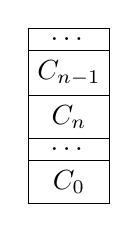
\begin{tikzpicture}[stack/.style={rectangle split, rectangle split parts=#1,draw, anchor=center}]
\node[stack=5]  {
\nodepart{one}$\dots$
\nodepart{two}$C_{n-1}$
\nodepart{three}$C_{n}$
\nodepart{four}$\dots$
\nodepart{five}$C_0$
};
\end{tikzpicture}
\par 
Par récurrence, si la pile est
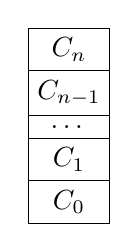
\begin{tikzpicture}[stack/.style={rectangle split, rectangle split parts=#1,draw, anchor=center}]
\node[stack=5]  {
\nodepart{one}$C_n$
\nodepart{two}$C_{n-1}$
\nodepart{three}$\dots$
\nodepart{four}$C_1$
\nodepart{five}$C_0$
};
\end{tikzpicture}
alors, le chemin allant de c0 a cn est [c0,c1,...,cn] Or $C_0 = (0,0)$, donc pour $C_n = (n-1,n-1)$ le chemin est la pile.
\begin{itemize}
	\item Là aussi, nous avons besoin d'une fonction auxilliaire, $\mathtt{revdup}$. Elle prend en argument une pile et retourne une pile contenant les mêmes éléments, mais retournés.
	\item Nous introduisons une nouvelle variable pour le labyrinthe : $\mathtt{chemin}$. Elle est initialisée à $\mathtt{False}$, mais contiendra la liste des cases du chemin à la fin. Lors de l'exécution du $\mathtt{while}$ principal, un premier cas se présente. En effet, si la case $(n-1,n-1)$ est atteinte, c'est alors qu'un chemin a été construit. Nous vérifions alors que $\mathtt{chemin}$ est encore vide, puis la valeur du chemin est stocké dans $\mathtt{chemin}$ sous forme de pile.
	\item En sortie du $\mathtt{while}$, le code suivan permet de modifier $\mathtt{lislab}$ pour changer la couleur du chemin.
\begin{lstlisting}
	xp,yp = depiler(chemin)
    lislab[2*xp+1][2*yp+1] = cc
    while not est_vide(chemin):
        (x,y) = depiler(chemin)
        lislab[2*x+1][2*y+1] = cc
        lislab[x+xp+1][y+yp+1] = cc
        xp,yp = x,y
    return lislab
\end{lstlisting}
\end{itemize}
Nous obtenons donc le code suivant :
\begin{lstlisting}
## Variables importantes

cc = 12 #quelques couleurs...
cb = 15

def revdup(p):
    """Prend en argument la pile p
    retourne une pile similaire à p et
    une pile contenant p retournée"""
    n = taille(p)
    s,t = creer_pile(n),creer_pile(n)
    for i in range(n):
        v = depiler(p)
        empiler(s,v)
        empiler(t,v)
    for j in range(n):
        empiler(p,depiler(s))
    return t
    
def labyrinthe():
    # Création de lislab, tableau de dimensions (2*n+1)
    #contenant la représentation du labyrinthe
    
    lislab = [[0]*(2*n+1) for i in range(2*n + 1)]
    
    for i in range(n):
        for j in range(n):
            lislab[2*i+1][2*j+1] = cb
            
    pile = creer_pile(n*n)
    chemin = False
    
    empiler(pile, (0,0))
    visiter((0,0))
    
    while not est_vide(pile):
        cellule = depiler(pile)
        
        #construction du chemin à la volée
        if cellule == (n-1,n-1) and not(chemin):
            empiler(pile,cellule)
            chemin = revdup(pile)
            cellule = depiler(pile)
            print(taille(chemin))
        
        #print(cellule)
        c = choix(cellule)
        if len(c) > 0:
            suivante = tirage(c)
            # Lie les deux cases
            xc,yc = cellule
            xs,ys = suivante
            #lislab[cellule[0] +1+ suivante[0]][cellule[1]+1 +suivante[1]] = cb
            lislab[xc+xs+1][yc+ys+1]=cb
            visiter(suivante)      
            empiler(pile, cellule)
            empiler(pile, suivante)
        # fin du while
        
    #ajout du chemin a lislab 
    xp,yp = depiler(chemin)
    lislab[2*xp+1][2*yp+1] = cc
    while not est_vide(chemin):
        (x,y) = depiler(chemin)
        lislab[2*x+1][2*y+1] = cc
        lislab[x+xp+1][y+yp+1] = cc
        xp,yp = x,y
    return lislab
\end{lstlisting}
\end{document}